%
% teil2.tex -- Beispiel-File für teil2 
%
% (c) 2020 Prof Dr Andreas Müller, Hochschule Rapperswil
%
% !TEX root = ../../buch.tex
% !TEX encoding = UTF-8
%
%https://blogs.mathworks.com/cleve/2013/10/14/complex-step-differentiation/

\section{Complex-Step-Differentiation}
\label{step:section:complex}
\kopfrechts{Complex-Step-Differentiation}

Neben der automatischen Differentiation mit dualen Zahlen existiert eine weitere numerische Methode zur präzisen Bestimmung von Ableitungen: die \emph{Complex-Step-Differentiation}.  
Diese Methode kombiniert die Vorteile numerischer Verfahren mit einer deutlich höheren Genauigkeit als die klassische finite Differenzenmethode.

Ausgangspunkt ist die Erweiterung reeller Funktionen auf den komplexen Zahlenraum. Sei dazu $f:\mathbb{R} \to \mathbb{R}$ eine holomorphe Funktion, die sich analytisch auf $\mathbb{C}$ fortsetzen lässt.  
Wird nun das Argument der Funktion um einen rein imaginären Anteil erweitert, ergibt sich

\begin{equation*}
	f(x + i h),
\end{equation*}
wobei $i$ die imaginäre Einheit mit $i^2 = -1$ ist und $h \in \mathbb{R}$ wiederum eine kleine Schrittweite darstellt.

\subsection{Herleitung der Methode}

Nimmt man die Taylorentwicklung (\ref{step:taylor2}) und evaluiert diese am komplexwertigen Punkt $x + ih$ ergibt sich

\begin{equation*}
	f(x + i h) = f(x) + i h f'(x) - \frac{h^2}{2} f''(x) - i \frac{h^3}{6} f^{(3)}(x) + \frac{h^4}{24} f^{(4)}(x) + \dots .
\end{equation*}
Betrachtet man nun den Imaginärteil dieses Ausdrucks, so ergibt sich

\begin{equation*}
	\Im(f(x + i h)) = h f'(x) - \frac{h^3}{6} f^{(3)}(x) + \dots .
\end{equation*}
Unter der Annahme, dass $h$ klein ist, kann die Reihe nach dem ersten Glied abgeschnitten werden, was zu folgendem Ausdruck für die Ableitung erster Ordnung führt

\begin{equation}
	f'(x) \approx \frac{\Im(f(x + i h))}{h}.
	\label{step:complexstep}
\end{equation}
Im Gegensatz zur finiten Differenzenmethode (\ref{step:finitdiff}) tritt hier kein Subtraktionsterm der Form $f(x+h) - f(x)$ auf.  %\label{step:finitdiff}
So wird verhindert, dass bei sehr kleinen Schrittweiten Auslöschungen auftreten, die sonst zu erheblichen Rundungsfehlern führen können.

\subsection{Anwendung der Complex-Step Methode}

Im Folgenden wird die Methode an zwei Funktionen getestet, einer Polynomfunktion sowie einer analytischen Funktion. 
In beiden Fällen wird gezeigt, dass die Methode in der Lage ist, die erste Ableitung nahezu fehlerfrei zu approximieren.
\paragraph{Beispiel\,1}
Gegeben sei das Polynom $f(x) = x^3 + x^2 + x + 1$, wobei dieses nun durch die Substitution $x \rightarrow x + ih$ erweitert wird. 
Es ergibt sich:
\begin{align*}
	f(x + ih) &= (x + ih)^3 + (x + ih)^2 + (x + ih) + 1 \\
	&= \big(x^3 + 3x^2ih + 3x(ih)^2 + (ih)^3\big) \\
	&\quad + \big(x^2 + 2xih + (ih)^2\big) + x + ih + 1 \\
	&= x^3 + 3x^2 ih + 3x(i^2 h^2) + i^3 h^3 \\
	&\quad + x^2 + 2x ih + i^2 h^2 + x + ih + 1 \\
	&= x^3 + 3x^2 ih - 3x h^2 - i h^3 \\
	&\quad + x^2 + 2x ih - h^2 + x + ih + 1 \\
	&= \big(x^3 + x^2 + x + 1 - 3x h^2 - h^2\big) \\
	&\quad + i\big(3x^2 h + 2x h + h - h^3\big)
\end{align*}
Zur Approximation der Ableitung wird der Imaginärteil betrachtet
\begin{align*}
	f'(x) \approx \frac{\Im(f(x + i h))}{h}
	&= 3x^2 + 2x + 1 - h^2.
\end{align*}
Für ein sehr kleines $h$ kann der Fehlerterm $h^2$ vernachlässigt werden, sodass sich für die Ableitung folgende Lösung ergibt
\begin{equation*}
f'(x) \approx 3x^2 + 2x + 1.
\end{equation*}
Damit zeigt sich, dass die Complex-Step Methode die exakte Ableitung ohne Subtraktionsfehler liefert.
Wie in Abbildung~\ref{fig:complex_step_fehler1} zu erkennen ist, liefert die Complex-Step-Methode im Vergleich zur Finite-Differenzen-Methode eine deutlich höhere Genauigkeit.
\begin{figure}[h!] %todo
	\centering
	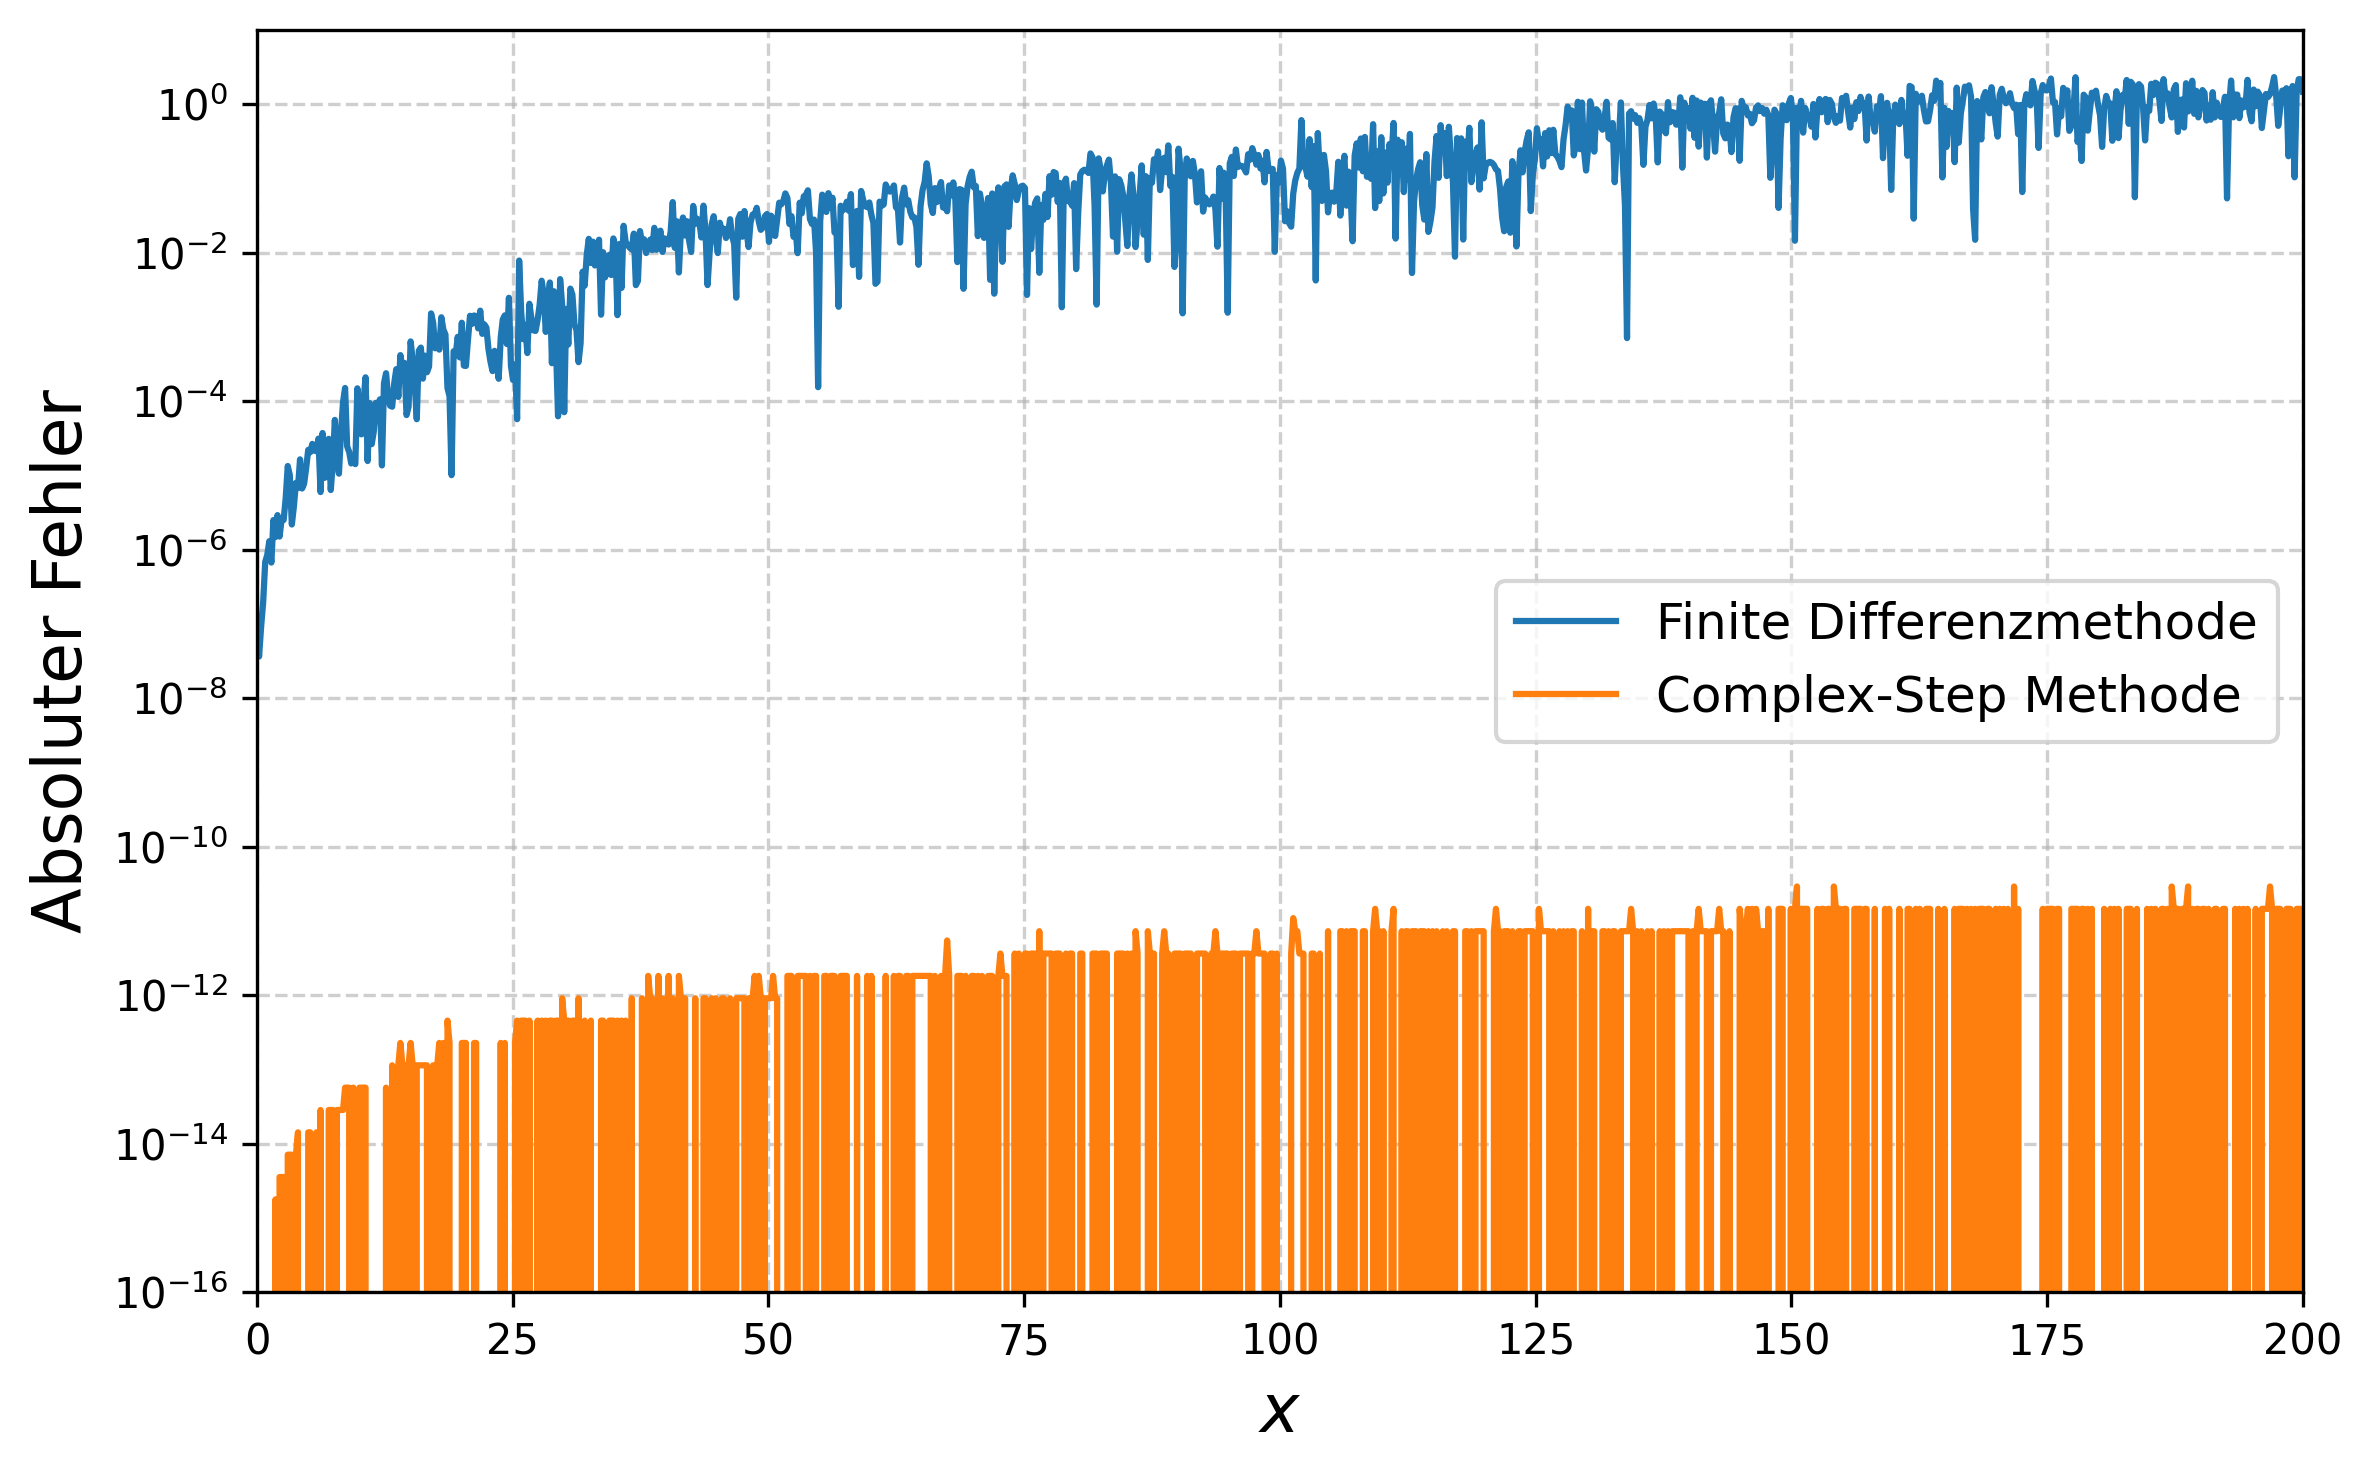
\includegraphics[width=0.8\textwidth]{papers/step/img/complex_step_vergleich1.png}
	\caption{Absoluter Fehler der Ableitung von $f(x) = x^3 + x^2 + x + 1$ 
		für Finite-Differenzen- und Complex-Step-Methode mit einer Schrittweite $h=10^{-9}$.}
	\label{fig:complex_step_fehler1}
\end{figure}
\paragraph{Beispiel\,2}
Gegeben sei die analytische Funktion $f(x) = \sin(x)$. Mittels Erweiterung in die komplexe Ebene $x + ih$ ergibt sich
\begin{align*}
	f(x + ih) &= \sin(x + ih) \\
	&= \sin(x)\cos(ih) + \cos(x)\sin(ih).
\end{align*}
Mithilfe der Kleinwinkelnäherungen $\cos(ih) \approx 1$ und $\sin(ih) \approx ih$ für kleine $h$ lässt sich obiger Ausdruck vereinfachen zu
\begin{equation*}
	f(x + ih) = \sin(x) + ih\cos(x).
\end{equation*}
Zur Approximation der Ableitung wird der Imaginärteil betrachtet
\begin{align*}
f'(x) \approx \frac{\Im(f(x + i h))}{h}
	&=\cos(x).
\end{align*}
Somit ergibt sich auch für diese Funktion eine präzise Bestimmung der Ableitung ohne numerisch bedingte Subtraktionsfehler, was durch die in Abbildung~\ref{fig:complex_step_fehler2} dargestellten Ergebnisse bestätigt wird.
\begin{figure}[h!] %todo
	\centering
	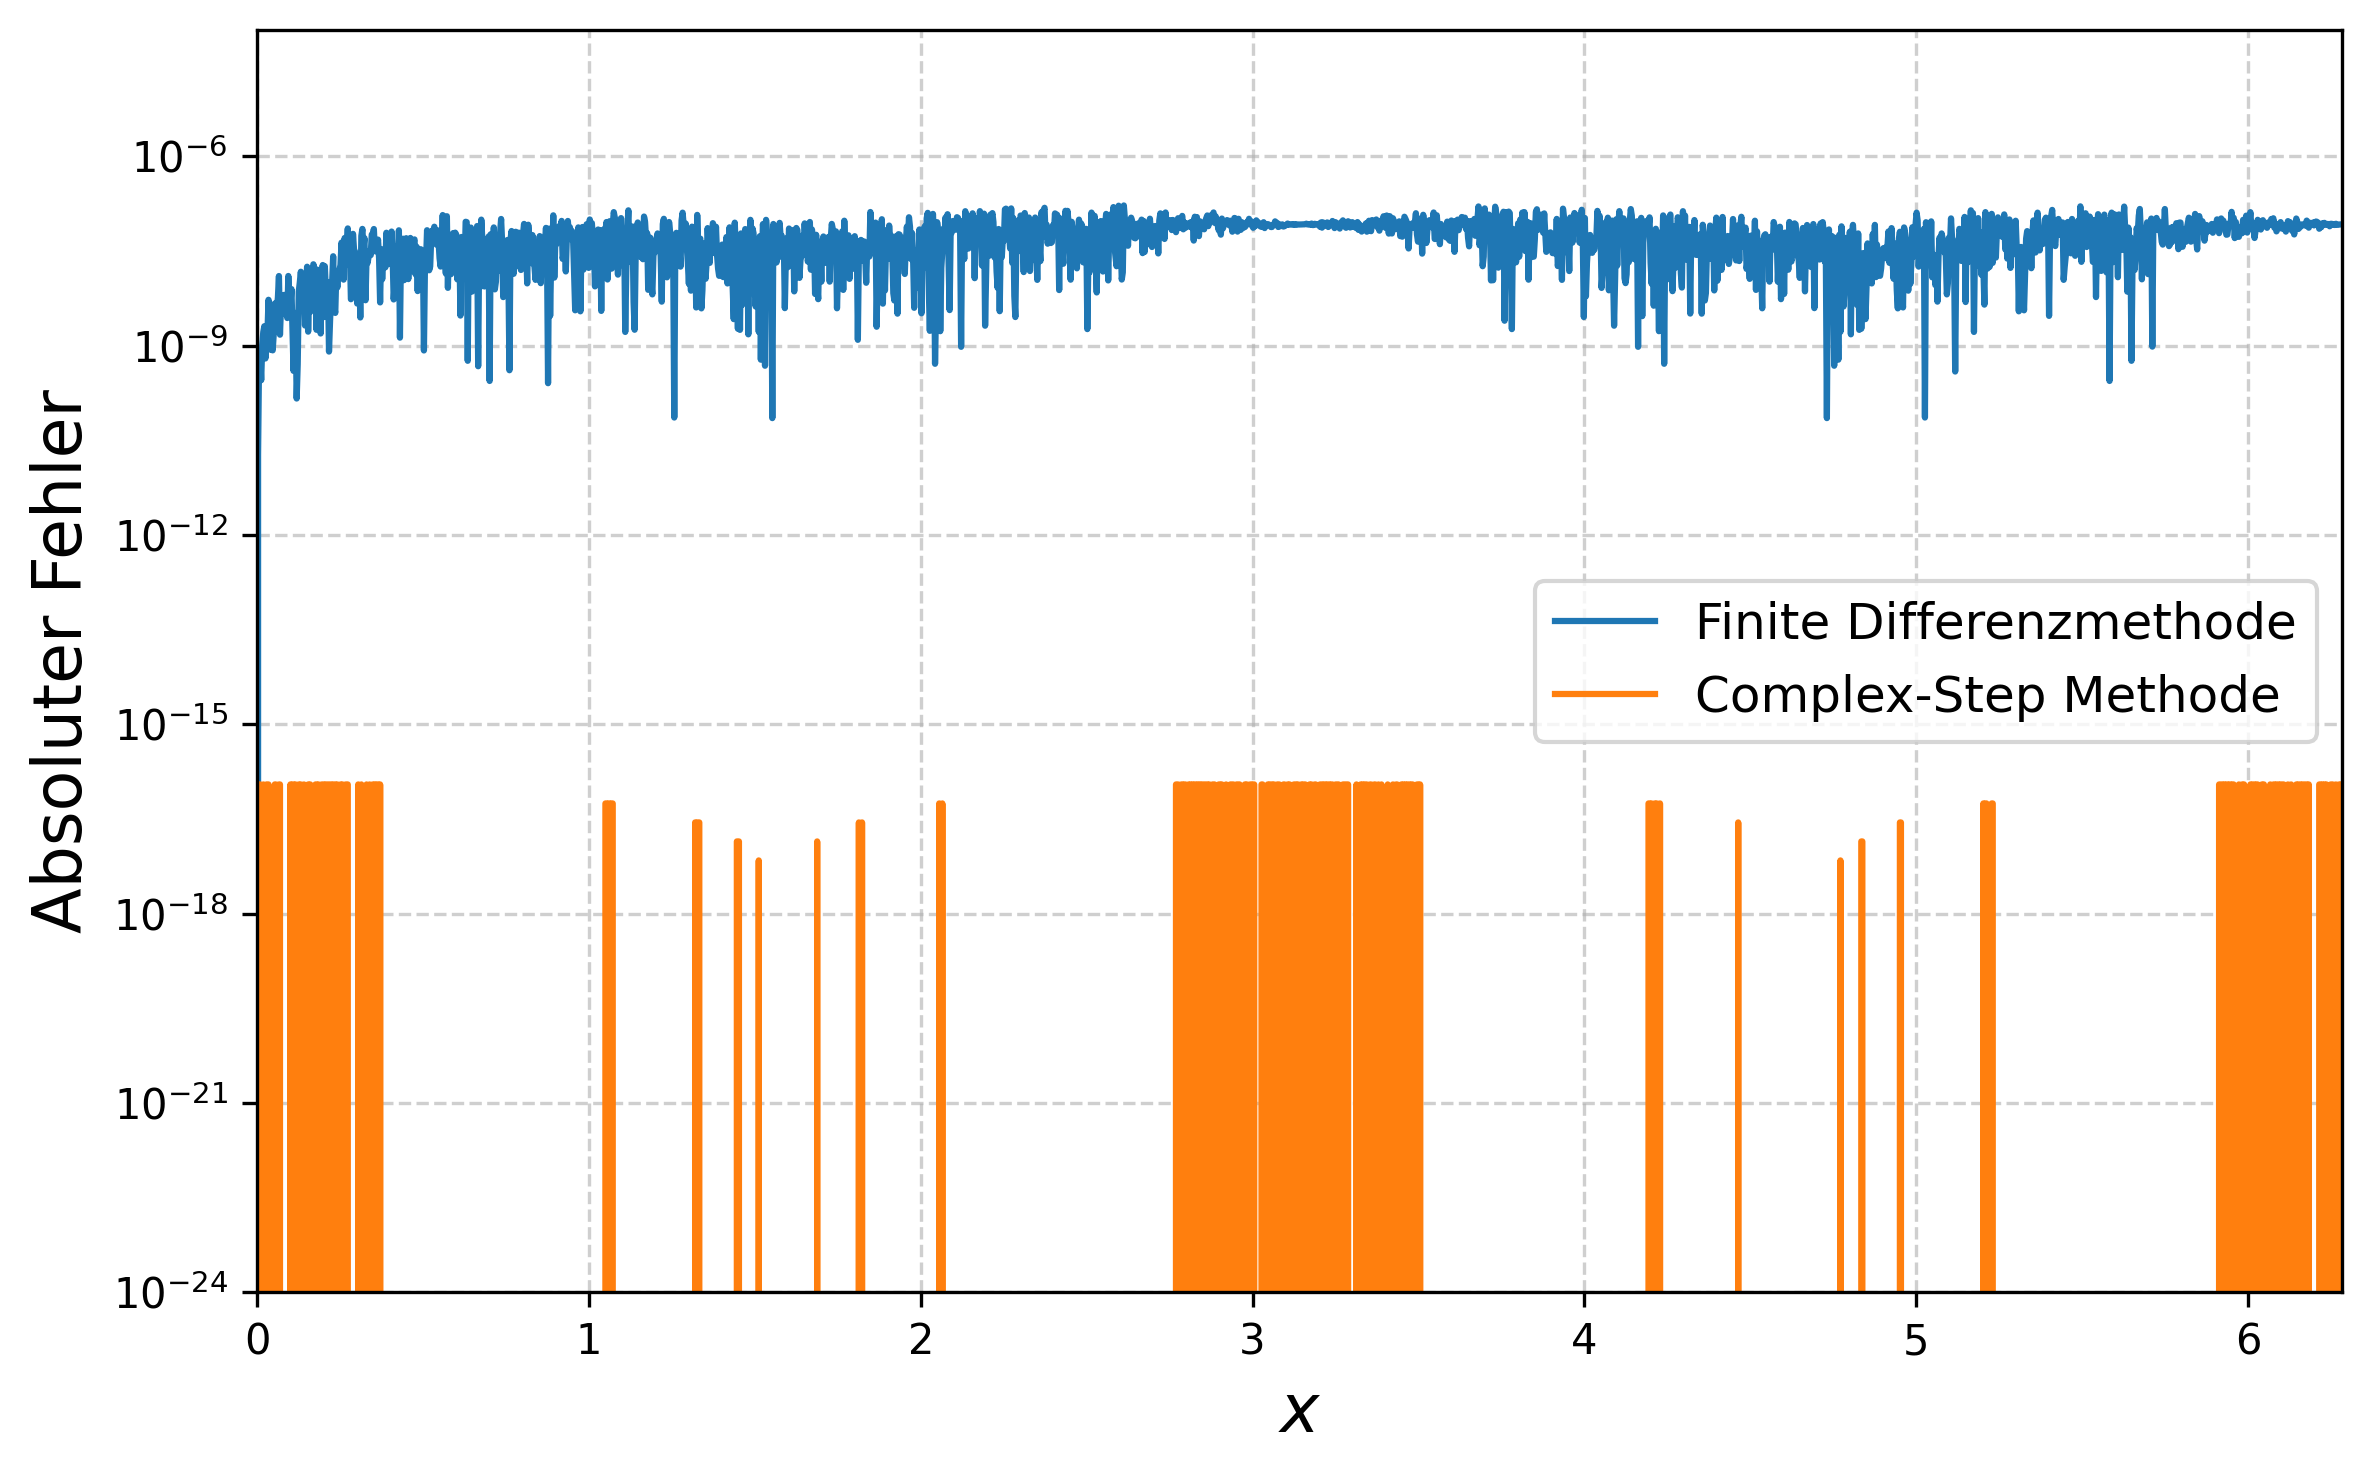
\includegraphics[width=0.8\textwidth]{papers/step/img/complex_step_vergleich2.png}
	\caption{Absoluter Fehler der Ableitung von $f(x) = \sin(x)$ 
		für Finite-Differenzen- und Complex-Step-Methode mit einer Schrittweite $h=10^{-9}$.}
	\label{fig:complex_step_fehler2}
\end{figure}

\subsection{Implementierung in Python}

Die Methode lässt sich in Python äußerst einfach implementieren, da komplexe Zahlen nativ unterstützt werden:

\begin{lstlisting}[
	numbers=none,
	basicstyle=\ttfamily\fontsize{7}{9}\selectfont,
	keepspaces=true,
	]
def complex_step(f, x, h=1e-20):
  return (f(x + 1j*h)).imag / h
\end{lstlisting}

\noindent Beispiel für die Ableitung der Sinusfunktion:

\begin{lstlisting}[
	numbers=none,
	basicstyle=\ttfamily\fontsize{7}{9}\selectfont,
	keepspaces=true,
	]
import math

def f(x):
  return math.sin(x)

>>> complex_step(f, 2*math.pi)
1.0
\end{lstlisting}
Im Vergleich ergibt sich mit der finiten Differenzenmethode:
\begin{lstlisting}[
	numbers=none,
	basicstyle=\ttfamily\fontsize{7}{9}\selectfont,
	keepspaces=true,
	]
>>> forward_diff(math.sin, 2*math.pi, 1e-12)
1.000088900582341
\end{lstlisting}
Das Ergebnis zeigt deutlich, dass die Complex-Step-Methode eine wesentlich höhere Genauigkeit liefert.

\subsection{Einordnung der Methode}

Die Complex-Step-Differentiation stellt einen Mittelweg zwischen der finiten Differenzenmethode und der automatischen Differentiation dar:

\begin{itemize}
	\item Im Gegensatz zur finiten Differenzenmethode ist sie numerisch stabil und nahezu exakt.
	\item Im Gegensatz zur automatischen Differentiation ist keine spezielle algebraische Struktur wie duale Zahlen erforderlich.
\end{itemize}

Allerdings existieren auch Einschränkungen:
\begin{itemize}
	\item Die Methode setzt voraus, dass die Funktion für komplexe Argumente definiert ist.
	\item Nicht alle numerischen Bibliotheken unterstützen komplexe Erweiterungen (z.\,B. manche optimierten Funktionen).
\end{itemize}

\subsection{Zusammenfassung}

Die Complex-Step-Differentiation ermöglicht eine äußerst präzise und numerisch stabile Berechnung erster Ableitungen.  
Durch die Verwendung komplexer Zahlen wird die Differenzbildung vermieden, wodurch Rundungsfehler drastisch reduziert werden.
Damit stellt sie eine leistungsfähige Alternative zur finiten Differenzenmethode dar und ergänzt die automatische Differentiation um einen weiteren praktischen Ansatz zur Ableitungsberechnung.

